%%%%%%%%%%%%%%%%%%%%%%%%%%%%%%%%%%%%%%%%%%%%%%%%%%%%%%%%%%%%%%%%%%%%%
%% This is a (brief) model paper using the achemso class
%% The document class accepts keyval options, which should include
%% the target journal and optionally the manuscript type. 
%%%%%%%%%%%%%%%%%%%%%%%%%%%%%%%%%%%%%%%%%%%%%%%%%%%%%%%%%%%%%%%%%%%%%
\documentclass[journal=jctcce,manuscript=article]{achemso}
%\documentclass[12pt]{article}
%\usepackage[letterpaper,left=0.5in,right=0.5in,top=1.0in,bottom=1.0in]{geometry}

%%%%%%%%%%%%%%%%%%%%%%%%%%%%%%%%%%%%%%%%%%%%%%%%%%%%%%%%%%%%%%%%%%%%%
%% Place any additional packages needed here.  Only include packages
%% which are essential, to avoid problems later. Do NOT use any
%% packages which require e-TeX (for example etoolbox): the e-TeX
%% extensions are not currently available on the ACS conversion
%% servers.
%%%%%%%%%%%%%%%%%%%%%%%%%%%%%%%%%%%%%%%%%%%%%%%%%%%%%%%%%%%%%%%%%%%%%
\usepackage[version=3]{mhchem} % Formula subscripts using \ce{}
\usepackage{siunitx} % generating degrees Celsius in the document 
\usepackage{color}
\usepackage{soul} % allows highlighting text 
\usepackage{makecell}
\usepackage{booktabs}



%%%%%%%%%%%%%%%%%%%%%%%%%%%%%%%%%%%%%%%%%%%%%%%%%%%%%%%%%%%%%%%%%%%%%
%% If issues arise when submitting your manuscript, you may want to
%% un-comment the next line.  This provides information on the
%% version of every file you have used.
%%%%%%%%%%%%%%%%%%%%%%%%%%%%%%%%%%%%%%%%%%%%%%%%%%%%%%%%%%%%%%%%%%%%%
%%\listfiles

%%%%%%%%%%%%%%%%%%%%%%%%%%%%%%%%%%%%%%%%%%%%%%%%%%%%%%%%%%%%%%%%%%%%%
%% Place any additional macros here.  Please use \newcommand* where
%% possible, and avoid layout-changing macros (which are not used
%% when typesetting).
%%%%%%%%%%%%%%%%%%%%%%%%%%%%%%%%%%%%%%%%%%%%%%%%%%%%%%%%%%%%%%%%%%%%%
\newcommand*\mycommand[1]{\texttt{\emph{#1}}}

%%%%%%%%%%%%%%%%%%%%%%%%%%%%%%%%%%%%%%%%%%%%%%%%%%%%%%%%%%%%%%%%%%%%%
%% Meta-data block
%% ---------------
%% Each author should be given as a separate \author command.
%%
%% Corresponding authors should have an e-mail given after the author
%% name as an \email command. Phone and fax numbers can be given
%% using \phone and \fax, respectively; this information is optional.
%%
%% The affiliation of authors is given after the authors; each
%% \affiliation command applies to all preceding authors not already
%% assigned an affiliation.
%%
%% The affiliation takes an option argument for the short name.  This
%% will typically be something like "University of Somewhere".
%%
%% The \altaffiliation macro should be used for new address, etc.
%% On the other hand, \alsoaffiliation is used on a per author basis
%% when authors are associated with multiple institutions.
%%%%%%%%%%%%%%%%%%%%%%%%%%%%%%%%%%%%%%%%%%%%%%%%%%%%%%%%%%%%%%%%%%%%%
\author{Stephen P. Vicchio}
\affiliation[Clemson University]
{Department of Chemical and Biomolecular Engineering, Clemson University, Clemson, SC}
\author{Sachi Hilliard}
\affiliation[Clemson University]
{Department of Chemical and Biomolecular Engineering, Clemson University, Clemson, SC}
%\author{Omar Farha?}
%\affiliation[Northwestern University]
%{Northwestern University}
\author{Rachel B. Getman}
\email{rgetman@g.clemson.edu}
\affiliation[Clemson University]
{Department of Chemical and Biomolecular Engineering, Clemson University, Clemson, SC}


%%%%%%%%%%%%%%%%%%%%%%%%%%%%%%%%%%%%%%%%%%%%%%%%%%%%%%%%%%%%%%%%%%%%%
%% The document title should be given as usual. Some journals require
%% a running title from the author: this should be supplied as an
%% optional argument to \title.
%%%%%%%%%%%%%%%%%%%%%%%%%%%%%%%%%%%%%%%%%%%%%%%%%%%%%%%%%%%%%%%%%%%%%
\title[manuscript]{Nickel(II) and Copper(II) Supported Metal Complex Stability in NU-1000 Under Hydrogenation Conditions}

%%%%%%%%%%%%%%%%%%%%%%%%%%%%%%%%%%%%%%%%%%%%%%%%%%%%%%%%%%%%%%%%%%%%%
%% Some journals require a list of abbreviations or keywords to be
%% supplied. These should be set up here, and will be printed after
%% the title and author information, if needed.
%%%%%%%%%%%%%%%%%%%%%%%%%%%%%%%%%%%%%%%%%%%%%%%%%%%%%%%%%%%%%%%%%%%%%
\abbreviations{IR,NMR,UV}
\keywords{American Chemical Society, \LaTeX}

%%%%%%%%%%%%%%%%%%%%%%%%%%%%%%%%%%%%%%%%%%%%%%%%%%%%%%%%%%%%%%%%%%%%%
%% The manuscript does not need to include \maketitle, which is
%% executed automatically.
%%%%%%%%%%%%%%%%%%%%%%%%%%%%%%%%%%%%%%%%%%%%%%%%%%%%%%%%%%%%%%%%%%%%%
\begin{document}

%%%%%%%%%%%%%%%%%%%%%%%%%%%%%%%%%%%%%%%%%%%%%%%%%%%%%%%%%%%%%%%%%%%%%
%% The "tocentry" environment can be used to create an entry for the
%% graphical table of contents. It is given here as some journals
%% require that it is printed as part of the abstract page. It will
%% be automatically moved as appropriate.
%%%%%%%%%%%%%%%%%%%%%%%%%%%%%%%%%%%%%%%%%%%%%%%%%%%%%%%%%%%%%%%%%%%%%
%\begin{tocentry}
%
%Some journals require a graphical entry for the Table of Contents.
%This should be laid out ``print ready'' so that the sizing of the
%text is correct.
%
%Inside the \texttt{tocentry} environment, the font used is %Helvetica
%8\,pt, as required by \emph{Journal of the American Chemical
%Society}.
%
%The surrounding frame is 9\,cm by 3.5\,cm, which is the maximum
%permitted for  \emph{Journal of the American Chemical Society}
%graphical table of content entries. The box will not resize if the
%content is too big: instead it will overflow the edge of the box.
%
%This box and the associated title will always be printed on a
%separate page at the end of the document.
%
%\end{tocentry}

%%%%%%%%%%%%%%%%%%%%%%%%%%%%%%%%%%%%%%%%%%%%%%%%%%%%%%%%%%%%%%%%%%%%%
%% The abstract environment will automatically gobble the contents
%% if an abstract is not used by the target journal.
%%%%%%%%%%%%%%%%%%%%%%%%%%%%%%%%%%%%%%%%%%%%%%%%%%%%%%%%%%%%%%%%%%%%%
\begin{abstract}
    
\end{abstract}

%%%%%%%%%%%%%%%%%%%%%%%%%%%%%%%%%%%%%%%%%%%%%%%%%%%%%%%%%%%%%%%%%%%%%
%% Start the main part of the manuscript here.
%%%%%%%%%%%%%%%%%%%%%%%%%%%%%%%%%%%%%%%%%%%%%%%%%%%%%%%%%%%%%%%%%%%%%
\newpage
\section{Introduction}

%\begin{figure}[t]
%    \centering
%    \includegraphics[width=0.95\textwidth]{zi-images/00-General-Graphics/2020-07-31-Combined-%MOF-Figure-final.png}
%    \caption{The structure of NU-1000, which is comprised of (a)  inorganic nodes %(\ce{[Zr6(\mu3-O)4(\mu3-OH)4(H2O)4(OH)4]^8^+}) and (b) organic linkers %(1,3,6,8-tetrakis(p-benzoic acid)pyrene (\ce{TBAPy^4^-})) to produce (c) the framework %structure (with the c-pore highlighted by the gray box). Additionally, the two metal %complexes supported in the c-pore of NU-1000 are also shown: (d) the \ce{Cu3(OH)4} metal %complex, and (d) the \ce{Ni4(OH)6} metal complex.}
%    \label{fig:MOFstructure}
%\end{figure}

% Paragraph 1: Knowledge gap related to the problem about knowing the precise structure of the active site (both when synthesized and then when activated)
\subsection{Paragraph 0}
 Catalysts are vital to the present and future of society, with currently 90\% of the world's consumer goods requiring a catalyst during manufacturing.\cite{Hagen2015} Most industrially relevant catalysts are heterogeneous because of their robustness to reaction conditions and ease of recovery. However, standard bulk heterogeneous catalysts suffer from poorly defined active sites that inhibit molecular understandings of the precise catalyst structure and catalytic mechanisms; this lack of knowledge has limited rational catalyst design for bulk metal catalysts. Over the last two decades, a new area of heterogeneous catalysis has emerged involving metal-organic frameworks (MOFs). MOFs, a porous material formed from inorganic nodes interconnected by organic linkers, function as both a heterogeneous catalysts and catalyst supports.\hl{REFERENCE} MOFs exhibit a diverse platform of tunable structures with well-defined active sites and chemical functionality thus making them an attractive material for single-atom catalysis. 
 % note to self.. I think the end of this paragraph is OKAY.. it's the beginning that needs work.

\subsection{Paragraph 1}
Within the scientific community, the \ce{Zr} based MOF NU-1000 is commonly used as a catalyst support for 3d metal complexes. Structurally, the NU-1000 MOF contains \ce{Zr} nodes interconnected by carbon based pyrene linkers to generate both large hexagonal channels (30 A), triangular channels (10 A), and small pores (8 A).(\hl{REFERENCE}) The staggered arrangement of protons forming \ce{OH}- and \ce{OH2}-ligand pairs on the node generate anchoring sites for 3d transition metals.\cite{Planas2014} Deposition of 3d transition metal atoms on MOF framework occurs in the vapor phase via atomic layer deposition (ALD) in MOFs (AIM) \hl{REFERENCE} and in condensed phase via solvothermal deposition in MOFs (SIM) \hl{REFERENCE}. The \ce{OH_{x}}-ligands within the small pore (\~8 A) of NU-1000 preferentially bind the metal species within the framework,\cite{Gallington2016,Rimoldi2017} and the synthesis conditions regulate the active species loading to generate complex active site structures.\cite{Kim2015} Elucidating the exact structure of the active site is challenging; characterization of the metal active sites is suppressed by the bulk framework structure, leading to questions about the structure and composition of the synthesized active site.

% Paragraph 2: More specific issue and problems 
% the different types of potential models for these systems.. there are different modeling choices that can be made for these systems.. talk about the different Ni(II) models comprised of a single Ni(II) atoms.. 
\subsection{Paragraph 2}
Combined experimental characterization and computational modeling has provided insights the active site structure for 3d transition metals supported on the standard NU-1000 MOF framework. The primary focus remains understanding the exact composition of the active site structure that are dependent on the number of metal species. A mononuclear (single-site) model was originally thought to be the active site structure for metals supported on NU-1000.\cite{Li2016sintering,AbdelMageed2019,Gallington2016} Mechanistic investigations into ethylene hydrogenation\cite{Shabbir2020} and propyne partial hydrogenation and isomerization\cite{Hackler2020} use a mononuclear model to high-throughout screen different metal species. \citeauthor{Shabbir2020} demonstrates the different proton tolopogies the mononuclear active site can adopt,\cite{Shabbir2020} while \citeauthor{Hackler2020} investigates two different \ce{H2} splitting pathways on a mononuclear active site.\cite{Hackler2020} A potential limitation of these findings, however, is the usage of a mononuclear model. The structure of the active site has been refined revealing that the metal species supported in the c-pore are more likely to be multinuclear (i.e., consisting of multiple metal species). Using difference envelope density (DED),\cite{Li2017} and differential pair distribution function (dPDF) analysis,\cite{PlateroPrats2017} the formation of multinuclear clusters within the c-pore has been established as the active site for NU-1000. A recent study by \citeauthor{Kim2020}  illustrates the multinuclearity of the active site by determining metal loading per node for different metal precursors.\cite{Kim2020} With metal complex deposition occurring only within the c-pore using the ALD process, metal loading greater than 2 metal atoms per node suggest an active site containing multiple metal atoms. Providing further insight to the multinuclear active site structure for \ce{Ni} complexes, \citeauthor{PlateroPrats2017} suggest the formation of tetranuclear heterobimetallic nanowires spanning the length of the c-pore with the cluster attached to two nodes.\citeauthor{PlateroPrats2017} For \ce{Cu} complexes, \citeauthor{Ikuno2017} proposes a similar trinuclear structure that also spans the c-pore of NU-1000. Experimentally, the nature of the active site for metal complexes on NU-1000 is multinuclear rather than mononuclear; however, the precise structure of the multinuclear active site remains unknown. 

\subsection{Paragraph 3}
Further complicating our understanding of the active site structure is the structural changes induced  by the reaction environment during both the activation step and the reaction steps. The activation environment, and therefore the structural changes, determine the reaction mechanism, such as dehydrogenation, hydrogenation, dimerization, oligomerization. The reaction environment includes both the temperature and gas phase species. \citeauthor{Kim2015} experimentally determined that the metal loading of \ce{In} deceased from  6 \ce{In} per node to 2 \ce{In} per node as the temperature increased from \SI{80}{Celsius} to \SI{200}{Celsius}.\cite{Kim2015} For ethylene hydrogenation, \citeauthor{Li2016sintering} proposes a mechanism on a mononuclear (single-site) \ce{Ni(II)} complex that is activated with \ce{H2} gas to form a \ce{Ni} hydride by removing a coordinated \ce{OH}-ligand.\cite{Li2016sintering} In a similar \ce{H2} environment, \citeauthor{Halder2020} experimentally demonstrated that above \SI{200}{Celsius} the trinuclear \ce{Cu(II)}-clusters supported on NU-1000 are reduced to zero-valent \ce{Cu(0)} species and stripped away from the node with the NU-1000 framework reverting back to the original unit cell dimensions.\cite{Halder2020} Conversely, when exposed to similar reducing conditions the tetranuclear \ce{Ni(II)} cluster shows only subtle structural variations up to 200 oC\cite{PlateroPrats2017} suggesting the cluster is stable under these conditions and that the initial activation only produces subtle changes into the structure of the cluster. Proposed dimerization mechanisms on the tetranuclear \ce{Ni(II)} cluster activate with \ce{Et2AlCl} to remove \ce{OH}-ligands within the cluster as coordinated \ce{H2O} species and generate the active \ce{C2H5}$^*$ species coordinated to the \ce{Ni} atoms.\cite{Ye2017} Using a mononuclar site \ce{Co} cluster, \citeauthor{Li2017} proposes an activation step involving \ce{O2} gas that removes a coordinated \ce{H2O} and alters the coordination environment of the \ce{Co} atom. The metal complexes supported on MOFs, here specifically NU-1000, demonstrate structural variations depending on reaction conditions. To further our understanding of these metal complex active site structures and design better catalysts, there is a need to understand the transformation of the active site structure depending on the reaction environment. 

\subsection{Paragraph 4}
Herein our work addresses questions related to the structural changes of the metal complex active site as a function of both temperature and gas phase conditions. By combining Density Functional Theory (DFT) calculations with gas phase empirical models, we investigate cluster stability under different gas phase conditions (\ce{H2}) and temperature. Modeling focuses on the \ce{Ni4(OH)6} cluster proposed by \citeauthor{PlateroPrats2017} and the \ce{Cu3(OH)4} cluster proposed by \cite{Ikuno2017}. Our results provide structural information about the types of changes exhibited by the cluster to establish more appropriate molecular models. 

%%%%%%%%%%%%%%%%%%%%%%%%%%%%%%%%%%%%%%%%%%%%%%%%%%%%%%%%%%%%%%%%%%%%%
%% Methodology
%%%%%%%%%%%%%%%%%%%%%%%%%%%%%%%%%%%%%%%%%%%%%%%%%%%%%%%%%%%%%%%%%%%%%

\newpage
\section{Methodology}
We use a multinuclear \ce{Ni(II)} as a model to investigate how the reaction conditions, such as temperature ($T$) and pressure ($P$), influence the structure and composition of a supported metal complex. The model \ce{Ni(II)} complex (shown in Figure \ref{fig:ref_Ni4_structure}) is located within the small pore of NU-1000. The process of \ce{H2} adsorption and dissociation generates new structures that are compositional different relative to the reference structure. The metal complex features \ce{OH^{*}} and \ce{M^{*}} sites and, when activated with molecular \ce{H2}, accept \ce{H} species. The \ce{OH^{*}} sites can accept a \ce{H} atom to form adsorbed \ce{H2O}, that can desorb into the gas phase depending on conditions. The \ce{M^{*}} sites can accept an \ce{H} atom to form a metal hydride (\ce{M-H}). All the aforementioned transformations are dependent on the partial pressure of \ce{H2} ($P_{H_2}$), the partial pressure of \ce{H2O} ($P_{H_{2}O}$), and the reaction temperature ($T$). We model the changes in cluster structure and composition as a function of reaction conditions by computing the free energy of compositionally different structures (with respect to the number of \ce{H^{*}}, \ce{OH^{*}} and \ce{M^{*}} species) relative to a reference structure. 

\begin{figure}
    \centering
    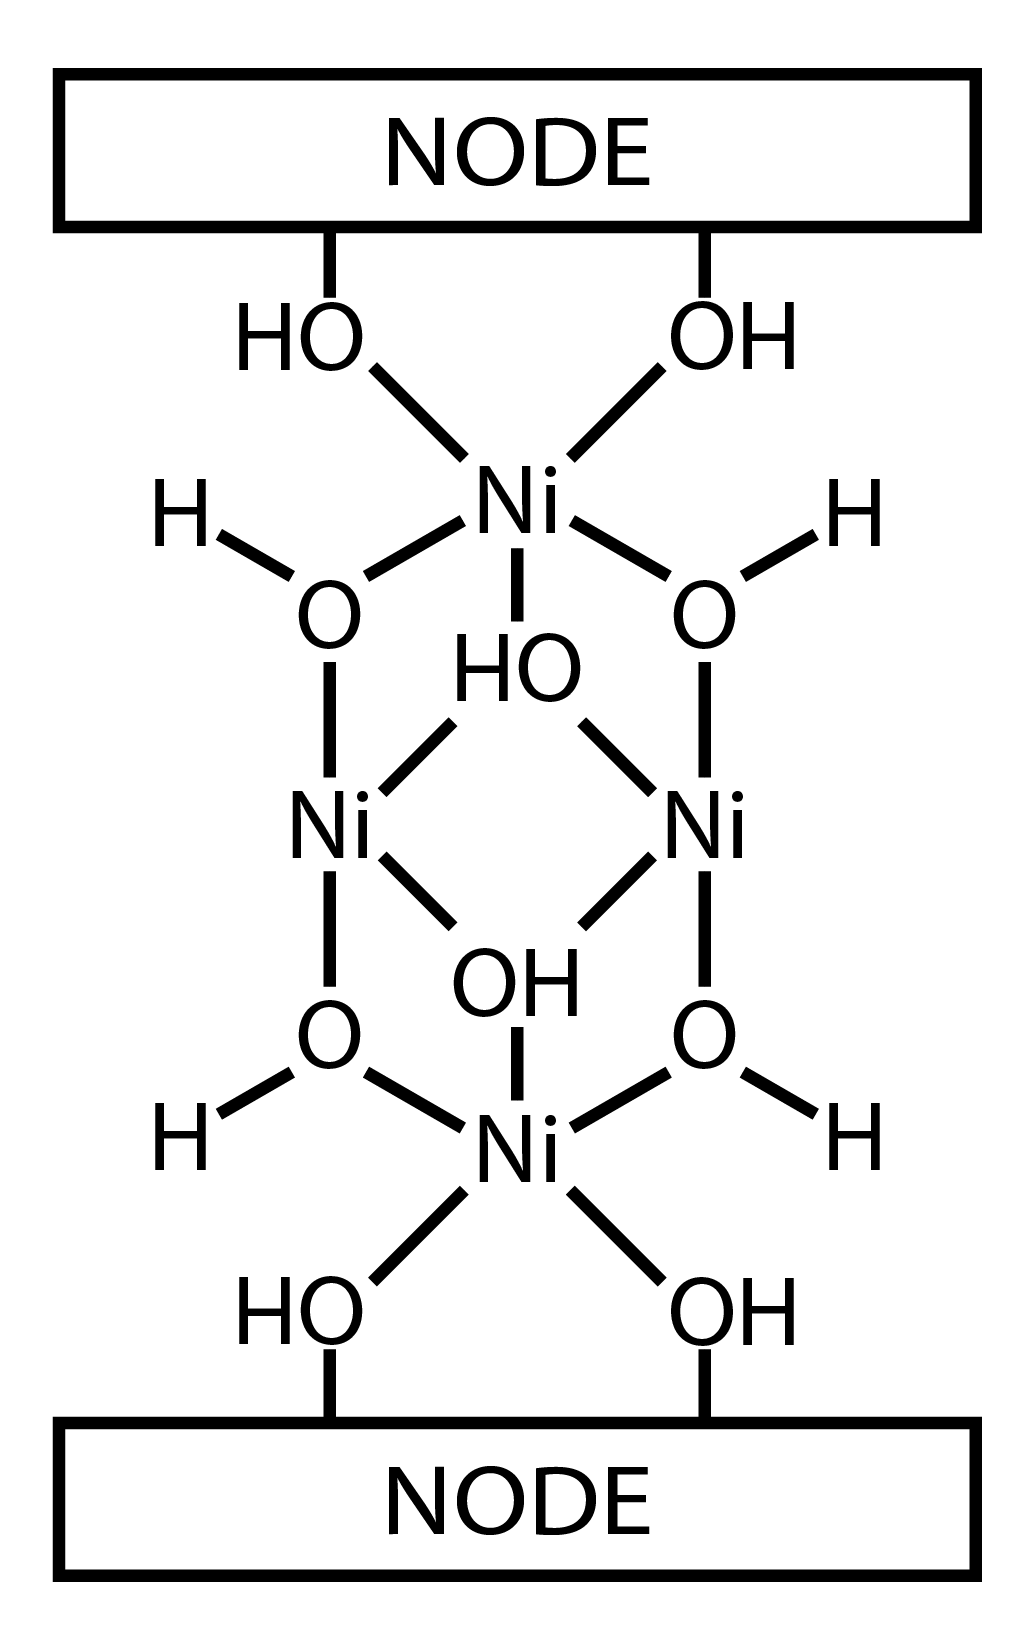
\includegraphics[width=0.20\textwidth]{zi-images/00-General-Graphics/Reference-structure.png}
    \caption{Structure of the multinuclear Ni(II) cluster supported on NU-1000. The cluster spans the small pore in NU-1000, and therefore attaches to two nodes. The structure is the reference for all \textit{ab initio} thermodynamic analysis calculations.}
    \label{fig:ref_Ni4_structure}
\end{figure}

We used \textit{ab initio} thermodynamic analysis to compute the stability of the different structural and compositional variations by transforming the free energy from a fixed number of atoms ($N_i$) to a fixed chemical potential ($\mu_i$). The free energy is transformed with respect to $\mu_{H^{*}}$, $\mu_{OH^{*}}$, and $\mu_{M^{*}}$ to account for structural and compositional variations in the number of \ce{H^{*}}, \ce{OH^{*}} and \ce{M^{*}} on the cluster (Figure \ref{fig:FPT-process}). Equation \ref{eq:free-energy-trans} shows the free energy difference ($ \Delta F^{(3)}(T,\mu_{H^{*}},\mu_{OH^{*}},\mu_{M^{*}})$) between structures $j$ and $i$ (see Supporting Information for the full derivation).
\begin{equation}
    \begin{split}
        \Delta F^{(3)}(T,\mu_{H^{*}},\mu_{OH^{*}},\mu_{M^{*}})  = 
        & F_{j}(T,N_{j,H^{*}},N_{j,OH^{*}},N_{j,M^{*}}) - 
          F_{i}(T,N_{i,H^{*}},N_{i,OH^{*}},N_{i,M^{*}}) \\
        & - (\mu_{H^{*}})(\Delta N_{H^{*}}) - (\mu_{OH^{*}})(\Delta N_{OH^{*}}) - (\mu_{M^{*}})(\Delta N_{M^{*}}) \\ 
    \end{split}
    \label{eq:free-energy-trans}
\end{equation}
The $F_{j}(T,N_{j,H^{*}},N_{j,OH^{*}},N_{j,M^{*}})$ term is the free energy of structure $j$ with configuration of $N_{j,H^{*}}$, $N_{j,OH^{*}}$, and $N_{j,M^{*}}$. The $\Delta N_{H^{*}}$, $\Delta N_{OH^{*}}$, and $\Delta N_{M^{*}}$ terms are the difference between $N_{j}$ and $N_{i}$ for that particular species. 

The chemical potential terms,  $\mu_{H^{*}}$ and $\mu_{OH^{*}}$, depend on the temperature and gas phase reaction conditions. We assume that $\ce{H^{*}}$ and $\ce{OH^{*}}$ are in equilibrium with an ideal-gas like reservoir with of \ce{H2} and \ce{H2O}, respectively (as shown in Figure \ref{fig:FPT-process}). The chemical potential of the reservoir is dependent on the reaction conditions ($T$ and $P$). The assumed equilibrium for $\ce{H^{*}}$ is with $\frac{1}{2}$ \ce{H2} (g) and for $\ce{OH^{*}}$ is with \ce{H2O} (g)/$\frac{1}{2}$\ce{H2} (g) (Equation \ref{eq:reaction_equilibrium}). The combined expression for $\ce{OH^{*}}$ captures the influence of both \ce{H2O} and \ce{H2} gas phase conditions on the stability of the cluster (further details in the Supporting Information).
\begin{equation}
    \begin{split}
        \frac{1}{2} H_{2} (g) & \ce{<=>} H^{*} \\           
        \frac{1}{2} H_{2} (g) + OH^{*} & \ce{<=>} H_{2}O (g)  
    \end{split}
    \label{eq:reaction_equilibrium}
\end{equation}
Using Equation \ref{eq:reaction_equilibrium}, the relationship between the $\ce{H^{*}}$ and $\ce{OH^{*}}$ species and the gas phase \ce{H2} and \ce{H2O} conditions are shown in Equation \ref{eq:chemicalpotentialeq}. The $\mu_{i}^{g}(T,P)$ terms contain the temperature and pressure influences of the reaction conditions. 
\begin{equation}
    \begin{split}
        \mu_{H^{*}} &= \frac{1}{2} \mu_{H_{2}}^{g}(T,P) \\ 
        \mu_{OH^{*}} &= \mu_{H_{2}O}^{g}(T,P) - \frac{1}{2} \mu_{H_{2}}^{g}(T,P) \\
    \end{split}
    \label{eq:chemicalpotentialeq}
\end{equation}
 The gas phase chemical potential terms ($\mu_{i}^{g}(T,P)$) are computed by correcting the electronic energy (referenced at $T$=0 K) of an isolated molecule  



with the gas-phase Gibbs free energy values at a specific temperature and pressure. The gas-phase Gibbs free energies ($\Delta G_{i}(T,P^{o})$) were computed using the NASA Polynomials\cite{Mcbride1993} in the pMuTT\cite{LYM2019106864} Python package at standard pressure ($P^{o}$) to capture the influence of temperature. The pressure effects ($P_{H_{2}}$ and $P_{H_{2}O}$) are captured assuming ideal gas for the gas phase species. The final expression for $\mu_{H_{2}}^{g}(T,P)$ and $\mu_{H_{2}O}^{g}(T,P)$ is given by Equation \ref{eq:chemicalpotentialrel}. 
\begin{equation}
    \begin{split}
        \mu_{H_{2}}^{g}(T,P) &= E_{H_2} + \Delta \mu_{H_{2}}(T,P)  = E_{H_{2}} + \Big[ \Delta G_{H_{2}}(T,P^{o}) + RT \ln{\Big( \frac{P_{H_{2}}}{P^{o}} \Big)} \Big] \\  
        \mu_{H_{2}O}^{g}(T,P) &= E_{H_{2}O} + \Delta \mu_{H_{2}O}(T,P^{o}) =  E_{H_{2}O} + \Big[ \Delta G_{H_{2}O}(T,P^{o}) + RT \ln{\Big( \frac{P_{H_{2}O}}{P^{o}} \Big)} \Big]
    \end{split}
    \label{eq:chemicalpotentialrel}
\end{equation}
The $\Delta \mu_{H_{2}}(T,P)$ and $\Delta \mu_{H_{2}O}(T,P^{o})$ 

Unlike the gas phase chemical potential terms, the metal chemical potential term ($\mu_{M^{*}}$) is independent of the reaction conditions and the metal chemical potential term assumed to be in equilibrium with a bulk metal system. The chemical potential $\mu_{M^{*}}$ is approximated by the electronic energy for a bulk metal system (see Supporting Information). 

Combining Equations \ref{eq:free-energy-trans}, \ref{eq:chemicalpotentialeq}, and \ref{eq:chemicalpotentialrel} produces the final transformed free energy expression (shown in the supporting information). The free energy expression was solved at every combination of $T$, $P_{H_2}$, and $P_{H_{2}O}$ for all structures. We generate a library of unique, modified structures for the \textit{ab initio} thermodynamic analysis by systematically adding \ce{H} atoms to different atoms on metal cluster and removing any formed \ce{H2O}. There are specific combinations of \ce{H^{*}}, \ce{OH^{*}} and \ce{M^{*}} within the library. At all combinations of $T$, $P_{H_2}$, and $P_{H_{2}O}$, the lowest free energy structure was identified thereby revealing the thermodynamic landscape of the modified metal cluster under reducing conditions. 

\begin{figure}[h]
    \centering
    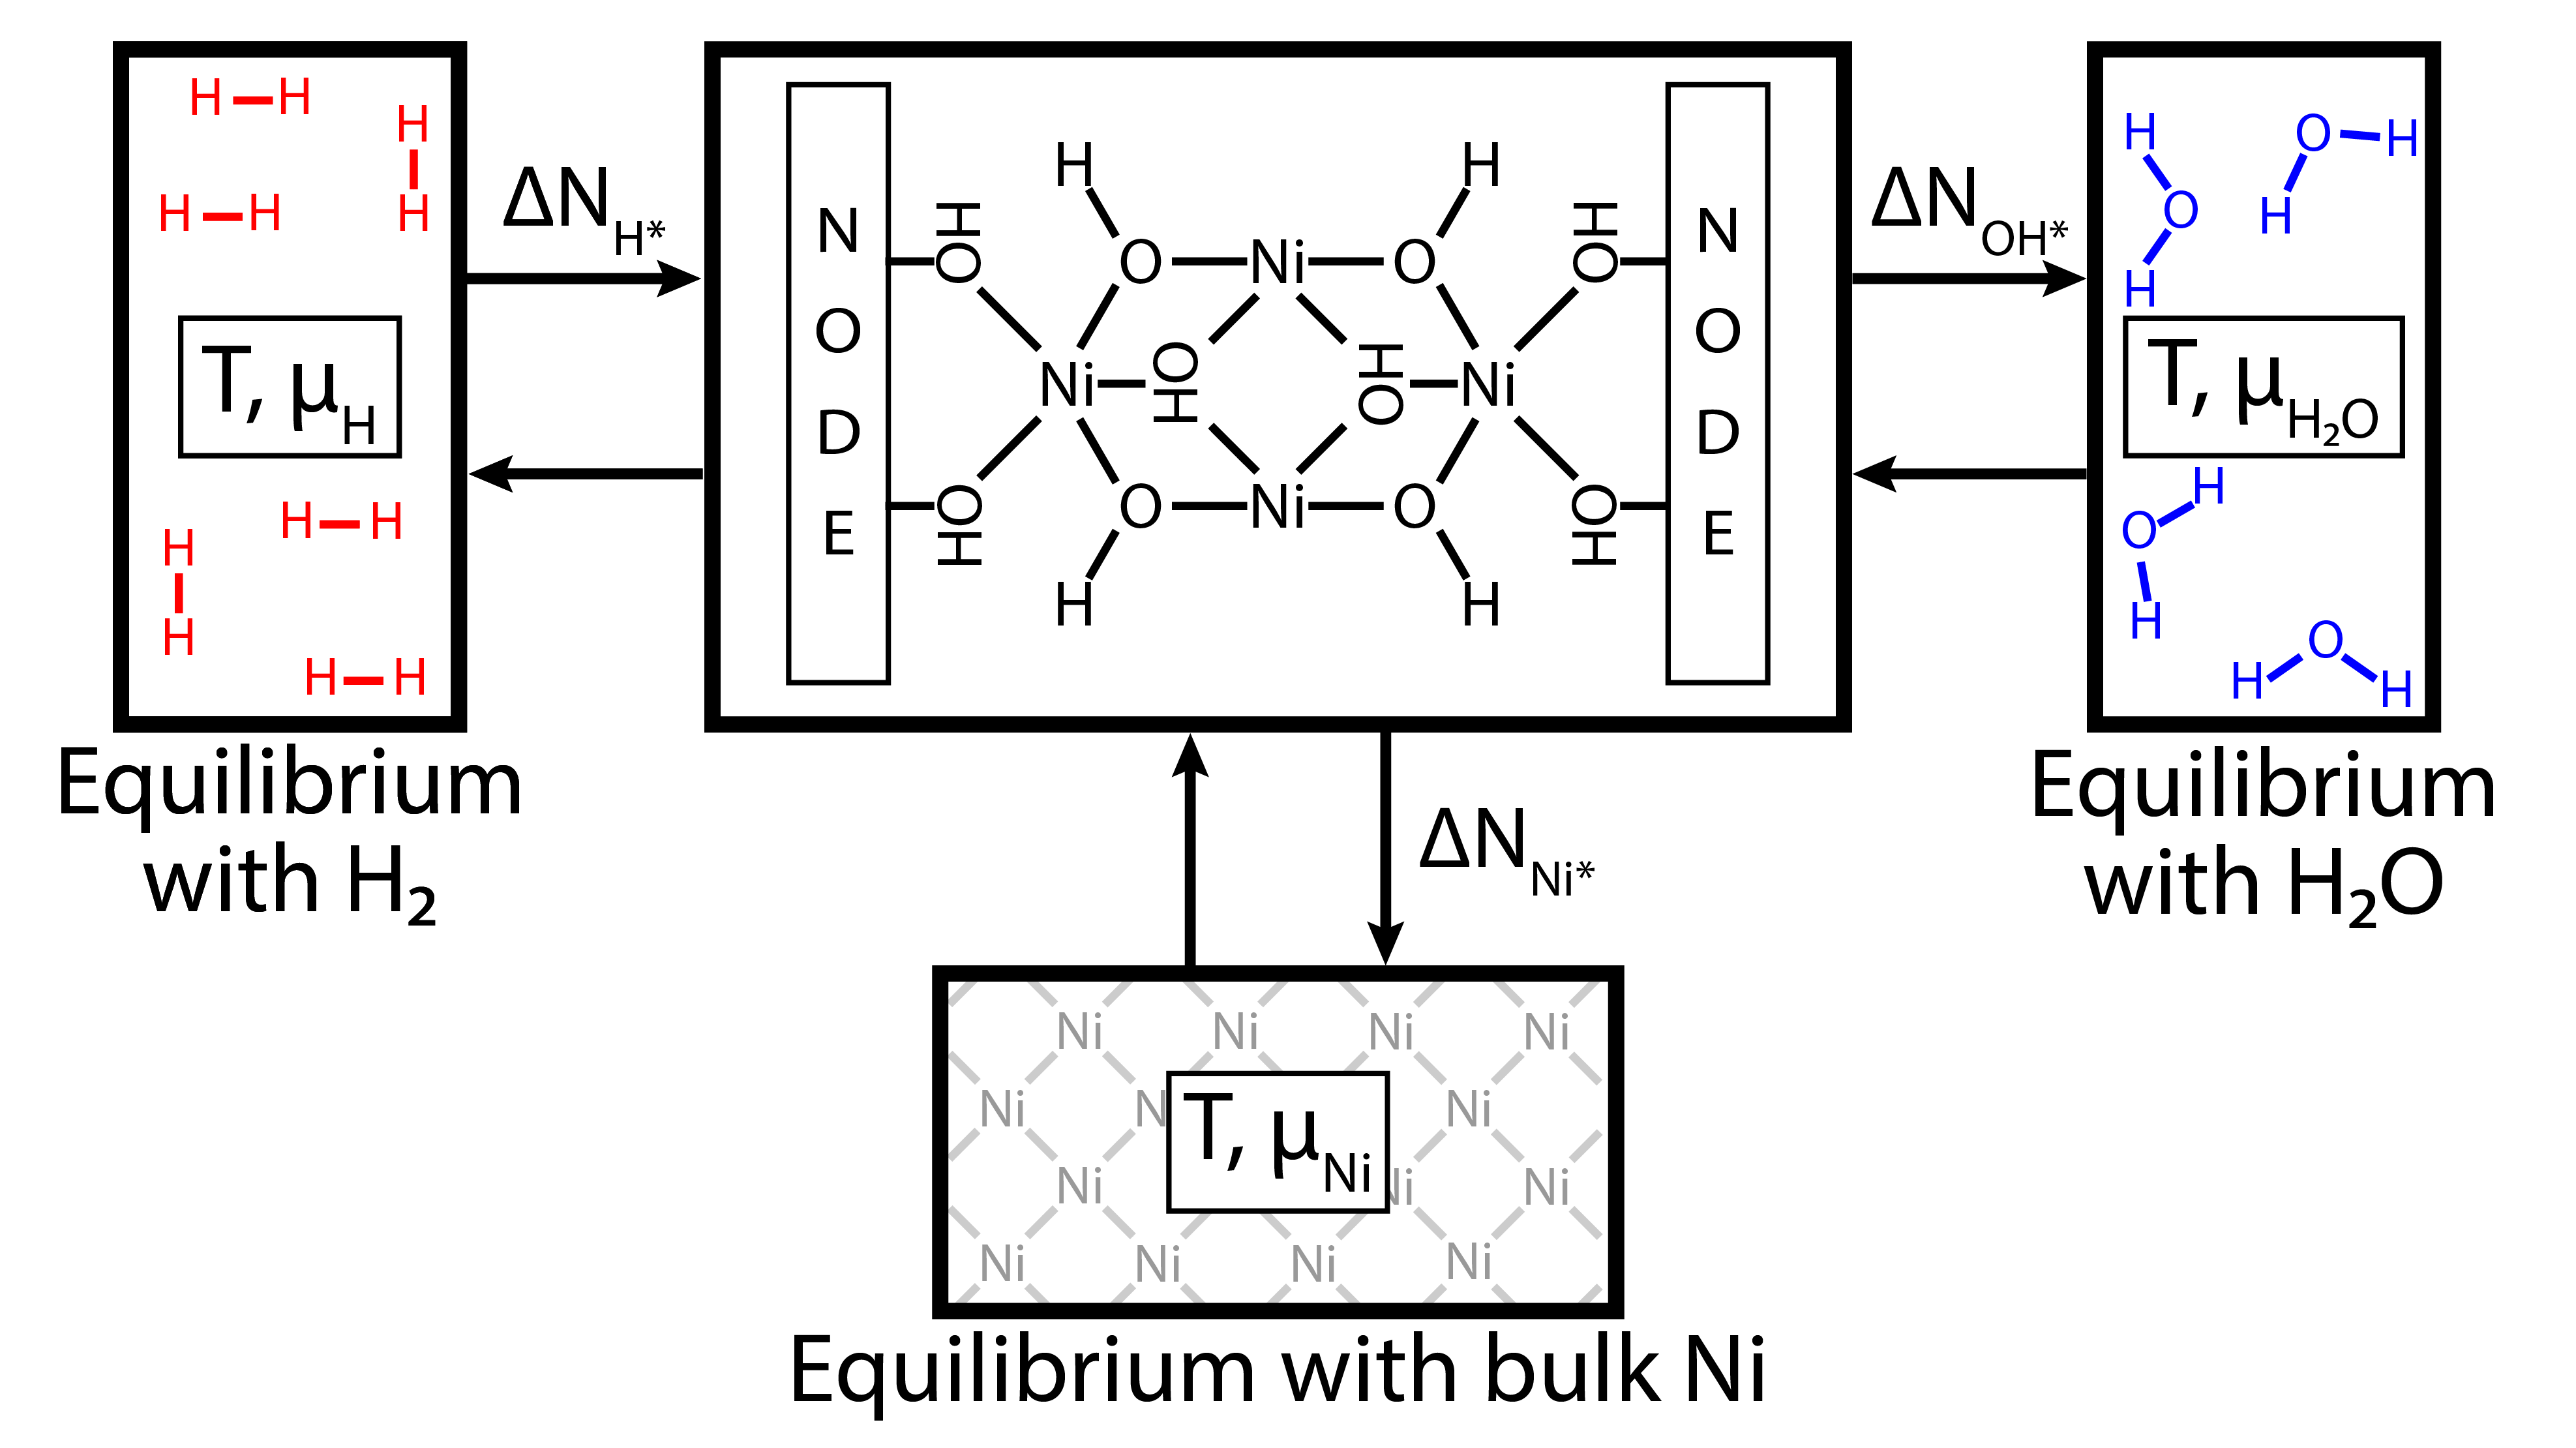
\includegraphics[width=0.85\textwidth]{zi-images/00-General-Graphics/FPT-schematic-full.png}
    \caption{Diagram showing the assumed equilibria necessary to transform with \ce{H^{*}}, \ce{OH^{*}}, and \ce{M^{*}} in the \textit{ab initio} thermodynamic analysis approach. The assumed equilibria for these adsorbed species capture the the reaction conditions on the stability of the metal cluster when using Equation \ref{eq:free-energy-trans}.}
    \label{fig:FPT-process}
\end{figure}

The energies for the structures are from periodic density functional (DFT) calculations in CP2K.\cite{Hutter2014} The exchange correlation energy was calculated with the PBE functional\cite{Perdew1996} and corrected using damped D3 dispersion corrections formulated by \citeauthor{Grimme2010}.\cite{Grimme2010} The DZVP-MOLOPT basis set describes the valance electrons, Goedecker pseudopotentials\cite{Goedecker1996} describes the core electrons. The plane wave cutoff energy is 360 Ry and  all atoms in the periodic unit cell were allowed to relax during geometry optimizations. \hl{A sample input file that contains the convergence criteria is located in the Supporting Information.} The variable spin states of the metal atoms required Unrestricted Kohn-Sham (UKS). For example, \ce{Ni(II)} can adopt both singlet (no unpaired electrons) and triplet (two unpaired electron) configurations. For clusters compromised of multiple metal atoms, all permutations of spin state configurations are simulated and included in the library of candidate structures. Any structures exhibiting spin contamination were removed from the analysis (see support information for more details).


%%%%%%%%%%%%%%%%%%%%%%%%%%%%%%%%%%%%%%%%%%%%%%%%%%%%%%%%%%%%%%%%%%%%%
%% Results
%%%%%%%%%%%%%%%%%%%%%%%%%%%%%%%%%%%%%%%%%%%%%%%%%%%%%%%%%%%%%%%%%%%%%
\newpage
\section{Results Outline}

\begin{itemize}
    \item Water content phase diagram. \hl{Insert the diagram that shows the water content as a function of T and partial pressure H2O.}
    \item Structure diagram for the content phase diagram. 
    \item Figure for phase diagram while transforming at fixed \ce{Ni(II)} content. 
        \begin{figure}
            \centering
        %    \includegraphics{}
            \caption{The stability of the \ce{Ni(II)} cluster at a function of temperature and \ce{H2} partial pressure at a \ce{H2O} partial pressure = $10^{-9}$ atm. Regions indicate the the modified structure that minimizes the free energy Equation (\ref{eq:free-energy-trans}) at a given combination of $T/P_{H_{2}}$ and fixed \ce{H2O} partial pressure. The name convention utilized to label each region is used throughout. The \ce{H2} partial pressure is reported as $log(P_{H_{2}}/P_{H_{2}}^{o})$, where the standard state is 1 atm.}
            \label{fig:phase_diagram_TandP}
        \end{figure}
    \item Figure for key structures on the phase diagram. 
    \item Figure now for transforming with \ce{H}, \ce{OH}, and \ce{Ni}. Draw the line the includes when accounting for removal of all \ce{Ni} atoms. Result shows that thermodynamically, the cluster is driven towards complete breakdown. The discussion will therefore suggest that ultimately the structure is driven towards complete breakdown. 
\end{itemize}



\newpage
\section{Results}
In this work, we show the stability of \ce{Ni(II)} and \ce{Cu(II)} clusters under reducing reaction conditions. The reference cluster is exposed to gaseous molecular \ce{H2} to induce structural changes on the cluster, which results in a modified structure. Phase diagrams show the stability of the cluster as a function of reaction temperature and \ce{H2} partial pressure at a fixed \ce{H2O} partial pressure. The \ce{H2O} partial pressure is {$10^{-13}$} atm, which is within the range of ultra high vacuum conditions \hl{REFERENCE FOR THESE CONDITIONS}. We do not expect a large \ce{H2O} partial pressure because gas phase \ce{H2O} species are formed from the removal of \ce{OH}-ligands in the cluster. Phase diagrams that vary the \ce{H2O} partial pressure can be found in the \hl{Supporting Information}. Figure \hl{XXX} shows the stability of the \ce{Ni(II)} cluster. 



We reduce the complexity of \ref{fig:phase_diagram_TandP} by defining two sets of reaction conditions to plot the free energy for all species in the \ce{Ni(II)} cluster library. The first set of conditions is at room temperature ($T = 20 ^{o}C$) and in the absence of \ce{H2} gas ($P_{H2}$ = \hl{XXX}) to show the stability of the cluster. The second set of conditions is activation conditions, with temperatures around $T = 200 ^{o}C$ and pressures around \hl{5\% H2 in 95\% (cite all the articles that activate with H2)}.      

%TODO: need to write the python script to show the differences... 
\begin{figure}
    \centering
%    \includegraphics{}
    \caption{The \ce{Ni(II)} cluster free energies are shown at different reaction conditions show. The number in parenthesis is the Boltzmann weighted average for that particular structure. Only structures within 50 $kJ/mol$ of the lowest energy structure are shown with the exact structures diagrams located in \hl{Supporting Information.}} The naming convention provides information on the structural features. 
    \label{fig:diff-reaction-conditons}
\end{figure}

%TODO: include the table that shows the reduction of the cluster. 

\begin{itemize}

    \item Reaction conditions are shown to depend on the gas phase conditions. 
    \item Phase Diagram 1: full transformation with of H*, OH*, M* 
    \begin{itemize}
        \item Phase diagram which show both T and PH2 that contains the correct structures. 
        \item Selecting a set of conditions and plotting the free energy of those structures along a set of conditions (think back to the line plots shown). Can generate the line plots at different conditions --> and then can use boltzmann weighting to determine the fraction of those structures at those conditions... 
        \item the most relevant structures that should be included on the diagram for this step. 
        \item need to select a partial pressure of H2O, which we will select as 10-10 to 10-15 because this is about the pressure for UHV..and I can plot the variation of this assumption in the SI for the paper to show. 
        \item Last statement..which will show in the SI a structure that contains the full cluster stripped away from MOFs... the phase diagram show the transformation of all Ni atoms away from the cluster
    \end{itemize}
\end{itemize}

%
%\subsection{Cu-NU-1000}
%
%\begin{figure}[H]
%    \centering
%    \includegraphics[width=0.95\textwidth]{zi-images/02-Cu-Graphics/2020-08-05-Cu3-ph%ase-diagram-V01.png}
%    \caption{Phase diagram generate by \textit{ab initio} thermodynamic analysis that %captures the structural stability of a Cu(II) supported metal complex in NU-1000 %at \SI{200}{\celsius}. The starting structure is the \ce{Cu3(OH)4} complex. The %composition and morphology of the Cu(II) complex changes depending on the \ce{H2} %and \ce{H2O} partial pressures, which produces new structural features, such as %physisorbed \ce{H2O} and metal hydride structures.}
%    \label{fig:phasediagramCu3}
%\end{figure}
%
%\begin{figure}[H]
%    \centering
%    \includegraphics[width=0.85\textwidth]{zi-images/02-Cu-Graphics/2020-08-04-struct%ure-diagram-Cu3OH4-V01-IMAGE.png}
%    \caption{Schematic representation of the lowest energy structures from the %\textit{ab initio} thermodynamic analysis. The node colors scheme correspond to %the \ce{Cu(II)} supported metal complex phase diagram (Figure %\ref{fig:phasediagramCu3}).}
%    \label{fig:structurediagramCu3}
%\end{figure}
%
%\begin{center}
%\begin{table}
%  \setlength\tabcolsep{8pt}
%  \caption{Copper Formal Charge State and \ce{Cu-Cu} Distances.}
%  \label{tbl:Cu3oxidationstates}
%  \begin{tabular}{lccc}
%    \hline
%        Structure  &  \thead{\ce{Cu} Formal \\ Charge\textsuperscript{\emph{a}}} &   %\thead{Potential \ce{Cu} \\ Oxidation State} & \thead{\ce{Cu-Cu} \\ Distance %(A)} \\
%        \hline
%        a) \ce{(CuHCuHCu)}                 & $\frac{4}{3}$ & \ce{Cu(0)}, \ce{Cu(II)}, %\ce{Cu(II)}       & 2.96, 3.10  \\
%        b) \ce{(CuHCu)(Cu)(OH)3}           & 2             & \ce{Cu(II)}, %\ce{Cu(II)}, \ce{Cu(II)}      & 2.81, 3.02  \\
%        c) \ce{(CuHCu)Cu(OH)3 \cdot 1H2O}  & 2             & \ce{Cu(II)}, %\ce{Cu(II)}, \ce{Cu(II)}      & 2.83, 3.03  \\
%        d) \ce{(CuCu)(Cu)}                 & $\frac{2}{3}$ & \ce{Cu(0)}, \ce{Cu(I)}, %\ce{Cu(I)}         & 2.37  \\
%        e) \ce{Cu3(OH)4}                   & 2             & \ce{Cu(II)}, %\ce{Cu(II)}, \ce{Cu(II)}      & 2.98, 3.02  \\
%        \hline
%    \end{tabular} \\
%    \textsuperscript{\emph{a}} Formal Charge given on a per Cu atom basis. \\
%\end{table}    
%\end{center}
%
%\begin{itemize}
%    \item The structure of \ce{Cu3(OH)4} complex is altered depending on the gas %phase conditions. The phase diagram for \ce{Cu3(OH)4} shows the formation of %physisorbed \ce{H2O} and \ce{Cu-H} species due to the adsorption and dissociation %of \ce{H2}. 
%    \begin{itemize}
%        \item The physisorbed \ce{H2O} species are formed by converting one of the %\ce{OH}-ligands in the cluster. The additional proton is from the adsorption %of the gas phase \ce{H2}. For \ce{Cu(OH)4}, the structure contains 4 %\ce{OH}-ligands that link the \ce{Cu} atoms across the c-pore. Figure %\ref{fig:phasediagramCu3} c) shows the the physisorbed \ce{H2O} and the %\ce{OH}-ligand replacement with an \ce{H} atom. Figure %\ref{fig:phasediagramCu3} shows how as the gas phase \ce{H2O} decreases, the %weakly bound \ce{H2O} molecule ( \ref{fig:structurediagramCu3} c)) desorbs %from the cluster (\ref{fig:structurediagramCu3} b)).
%        \item The \ce{Cu-H} species form when again by the dissociation of \ce{H2} on %the cluster. The phase diagram shows that as \ce{H2O} forms, the site %previously occupied by the \ce{OH}-ligand now contains the metal hydride %(\ce{Cu-H}). Interestingly, the metal hydrides that form 'bridge' two \ce{Cu} %atoms. Both \ref{fig:structurediagramCu3} a), b), and c) show the bridging %\ce{Cu-H-Cu} structures.
%    \end{itemize}
%    \item \ce{H2} partial pressure and \ce{H2O} partial pressure are important in the %structural stability. 
%    \begin{itemize}
%        \item The \ce{H2O} partial pressure can be used to inhibit the dissociative %adsorption of \ce{H2} (orange region on Figure \ref{fig:phasediagramCu3}).
%        \item As \ce{H2O} partial pressure decreases when exposed to \ce{H2}, the %cluster is reduced.
%    \end{itemize}
%    \item The two reduced structures (on Figure \ref{fig:phasediagramCu3} and Figure %\ref{fig:structurediagramCu3}) are \ce{(CuHCuHCu)} and \ce{(CuCu)(Cu)}. Both %structures show the conversion and removal of all \ce{OH}-ligands.
%    \begin{itemize}
%        \item \ce{(CuHCuHCu)} shows the complete reduction of \ce{Cu} and presence of %\ce{Cu-H-Cu} bridging structures. The bond distance seems too large for any %\ce{Cu-Cu} metallic bonds.  
%        \item \ce{(CuCu)(Cu)} shows the formation of a metallic \ce{Cu-Cu} bond (as %indicated by the 2.37 A. The \ce{Cu} atoms are not completely reduced, rather %exist as \ce{Cu(0)}, \ce{Cu(I)}, and \ce{Cu(I)}. This structure is %particularly interesting because it shows the formation of the mobile %\ce{Cu(0)} species. 
%    \end{itemize}
%    \item We are performing additional calculation that contains two mononuclear %(single-site) \ce{Cu} sites on both nodes in the c-pore with the middle \ce{Cu} %atom being removed. 
%\end{itemize}
%
%\begin{itemize}
%    \item structures a) and d) both generate the more mobile species.. structure a) %contained Cu-H-Cu bridge structures whereas d) generates Cu-Cu metal bonds.
%    \item structures b) and c) are analogous structures, except the partial pressure %of \ce{H2O} is sufficiently high, which can be used to prevent the desorption of %\ce{H2O} on the cluster. Both structures show the replacement of a hydroxo ligand %has been replaced with a metal hydride. For the multinuclear clusters, these %metal hydride structures are common. 
%    \item 
%\end{itemize}
% 
%\newpage
%\subsection{Ni-NU-1000}
%\begin{figure}[H]
%    \centering
%    \includegraphics[width=0.95\textwidth]{zi-images/01-Ni-Graphics/2020-08-31-Phase-%Diagram-V02.png}
%    \caption{Phase diagram generate by \textit{ab initio} thermodynamic analysis that %captures the structural stability of a Ni(II) supported metal complex in NU-1000 %at \SI{200}{\celsius}. The starting structure is the \ce{Ni4(OH)6} complex. The %composition and morphology of the Ni(II) complex changes depending on the \ce{H2} %and \ce{H2O} partial pressures, which produces new structural features, such as %physisorbed \ce{H2O} and metal hydride structures.}
%    \label{fig:phasediagramNi4}
%\end{figure}
%
%Figure \ref{fig:phasediagramNi4} shows the stability of the \ce{Ni4(OH)6} metal %complex under different hydrogenation conditions. As the partial pressure of \ce{H2} %increase (a more positive chemical potential) under ambient conditions, the %\ce{OH}-ligands within the \ce{Ni4(OH)6} metal complex are converted into physisorbed %\ce{H2O} through the dissociative adsorption of \ce{H2} onto the cluster. Increasing %the gas phase \ce{H2} partial pressure, increases the driving force for dissociative %adsorption. However, if the partial pressure of \ce{H2O} in the gas phase is too %large, the desorption of weakly bound \ce{H2O} molecules is prevented (as shown in %Figures \ref{fig:phasediagramNi4} and \ref{fig:structurediagramNi4}). Additionally, %\textit{ab initio} thermodynamic analysis suggests that at high enough partial %pressure of both \ce{H2O} and \ce{H2} that the cluster can exhibit both physisorbed %waters and metal hydride structures.
% 
%
%%At sufficient gas phase \ce{H2} partial pressures (e.g.\ log %$\frac{P_{\ce{H2}}}{P^{o}_{\ce{H2}}}=-1$ at \SI{200}{\celsius}), the cluster exhibits %dynamic structural changes in both morphology and composition. The changes show the %breakdown of the Ni(II) metal complex. Specifically, the the \ce{OH}-ligands are %systematically replaced by \ce{H} atoms that are forming metal hydride species. The %replacement of these \ce{OH}-ligands is clearly demonstrated in Figure %\ref{fig:structurediagramNi4}. These structural changes are further illustrated by %the reduction in the oxidation state of \ce{Ni} and the decreasing distance between %\ce{Ni} atoms (Table \ref{tbl:Ni4oxidationstates}). 
%
%\begin{table}
%  \setlength\tabcolsep{8pt}
%  \caption{Nickel Formal Charge and \ce{Ni-Ni} Bond Distances.}
%  \label{tbl:Ni4oxidationstates}
%  \begin{tabular}{lccc}
%    \hline
%        Structure  &  \thead{\ce{Ni} Formal \\ Charge\textsuperscript{\emph{a}}} &   % \thead{Potential \ce{Ni} \\ Oxidation State} & \thead{\ce{Ni-Ni} \\ Distance %(A)} \\
%    \hline 
%    a) \ce{(NiH2Ni)(NiNi)}             & 1             & \ce{Ni(0)}, \ce{Ni(I)}, %\ce{Ni(II)}, \ce{Ni(II)}     & 2.23, 2.42 \\   
%    b) \ce{(Ni3H2)(Ni)(OH)2}           & $\frac{3}{2}$ & \ce{Ni(I)}, \ce{Ni(I)}, %\ce{Ni(II)}, \ce{Ni(II)}     & 2.21, 2.54 \\ 
%    c) \ce{(NiH)(Ni3H)(OH)2 * 1H2O}    & $\frac{3}{2}$ & \ce{Ni(0)}, \ce{Ni(II)}, %\ce{Ni(II)}, \ce{Ni(II)}     & 2.27, 2.31 \\   
%    d) \ce{(Ni2)(NiH)2(OH)4 * 2H2O}    & 2             & \ce{Ni(II)}, \ce{Ni(II)}, %\ce{Ni(II)}, \ce{Ni(II)}     & 2.72, 3.17 \\     
%    e) \ce{(Ni2H)(NiNi)(OH)}           & 1             & \ce{Ni(0)}, \ce{Ni(I)}, %\ce{Ni(I)}, \ce{Ni(II)}     & 2.24, 2.50 \\  
%    f) \ce{Ni4(OH)4}                   & $\frac{3}{2}$ & \ce{Ni(I)}, \ce{Ni(I)}, %\ce{Ni(II)}, \ce{Ni(II)}   & 2.27, 3.06 \\
%    g) \ce{Ni4(OH)4 \cdot 1H2O}        & $\frac{3}{2}$ & \ce{Ni(I)}, \ce{Ni(I)}, %\ce{Ni(II)}, \ce{Ni(II)}   & 2.29, 2.96 \\
%    h) \ce{Ni4(OH)4 \cdot 2H2O}        & $\frac{3}{2}$ & \ce{Ni(I)}, \ce{Ni(I)}, %\ce{Ni(II)}, \ce{Ni(II)}   & 2.33, 3.03 \\
%    i) \ce{Ni4(OH)6}                   & 2             & \ce{Ni(II)}, \ce{Ni(II)}, %\ce{Ni(II)}, \ce{Ni(II)} & 2.81, 3.03 \\
%    \hline
%  \end{tabular} \\
%  \textsuperscript{\emph{a}} Formal Charge given on a per Ni atom basis. \\
%\end{table}
%
%%The replacement of structural \ce{OH}-ligands with \ce{H} atoms, the decreasing of %\ce{Ni} oxidation state, and the decreasing \ce{Ni-Ni} distances all suggests that %under these reducing conditions the \ce{Ni(II)} metal complex is no longer stable. %That is, thermodynamically, under these conditions the metal atoms of the supported %metal complex are being liberated, suggesting that the formation of \ce{Ni} %nanoparticles is favorable in this regime. The \ce{Ni(II)} atoms are reduced to %metallic \ce{Ni(0)}, supported by the formation of metallic \ce{Ni} bonds. 
%
%\begin{figure}[H]
%    \centering
%    \includegraphics[width=0.85\textwidth]{zi-images/01-Ni-Graphics/2020-08-31-Struct%ureDiagram-V01.png}
%    \caption{Schematic representation of the lowest energy structures from the %\textit{ab initio} thermodynamic analysis. The node colors scheme correspond to %the \ce{Ni(II)} supported metal complex phase diagram (Figure %\ref{fig:phasediagramNi4}).}
%    \label{fig:structurediagramNi4}
%\end{figure}
%
%\begin{itemize}
%    \item The \ce{Ni4(OH)6} phase diagram is structurally more diverse than the %\ce{Cu3(OH)4} phase diagram (attributed to more metal and \ce{OH}-ligands in the %\ce{Ni} metal complex). However, there are similar features as the \ce{Cu3(OH)4 %}(\ref{fig:phasediagramCu3}). Both demonstrate metal hydrides, and physisorbed %\ce{H2O}.
%    \item The presence of \ce{H2O} in the gas phase has a strong influence over the %structurally stability. For example, at \ce{H2} partial pressure of ~ $10^-1$ %bar, the reduction of the cluster is illustrated going from \ce{Ni2(NiH)2(OH)4} %to \ce{(NiH2Ni)(NiNi)}. At higher \ce{H2O} partial pressure, the cluster is more %likely to exist as a combination of \ce{Ni-H} and physisorbed \ce{H2O}. As the %partial pressure of \ce{H2O} decreases, the formed physisorbed \ce{H2O} is %removed. Overall, if the cluster is exposed to a sufficient \ce{H2} gas the %cluster is reduced. 
%    \item The main structures to focus on are the structures that demonstrate the %\ce{Ni} reduction from \ce{Ni(II)} to \ce{Ni(0)}. These structures reveal the %presence of metallic \ce{Ni} bonds (the more mobile species).
%\end{itemize}

%%%%%%%%%%%%%%%%%%%%%%%%%%%%%%%%%%%%%%%%%%%%%%%%%%%%%%%%%%%%%%%%%%%%%
%% Discussion
%%%%%%%%%%%%%%%%%%%%%%%%%%%%%%%%%%%%%%%%%%%%%%%%%%%%%%%%%%%%%%%%%%%%
\newpage
\subsection{Discussion}
The \ce{Ni(II)} metal complex structure is dependent on the environment. In the absence of any \ce{H2}, the cluster contains four \ce{Ni(II)} atoms interconnected by \ce{OH}-ligands as suggested by \hl{REFERENCE Platero-Prats}. The tetranuclear configuration of the \ce{Ni(II)} cluster spans the c-pore of the NU-1000 framework. When exposed to \ce{H2} gas, the \ce{OH}-ligands provide sites for \ce{H} adsorption onto the cluster resulting in the formation of \ce{H2O}.  \hl{HIGHLIGHT THE SINTERING PAPER} investigate \ce{H2} adsorption and dissociation on a single \ce{Ni} atom also supported on NU-1000, finding that barriers for \ce{H2} adsorption and dissociation and removal of \ce{H2O} are 141 $kJ/mol$. However within our work, we do not look at the kinetics of \ce{H2} adsorption and dissociation and the subsequent removal of \ce{H2O}. Our discussion focuses on the equilibrium thermodynamic structure resulting from exposure to \ce{H2} gas at different partial pressure and temperatures. 

% Paragraph on the inclusion of the reducing agent

% Paragraph about how we also decided to investigate Cu structure as well. 

% Paragraph on the breakdown of the chain structures and then suggestions on where those Ni atoms compared to the Cu atoms that form 

% Paragraph on the kinetic restraints

\begin{itemize}
    \item The structural characteristics of the supported metal complexes are dependent on the reaction conditions.
    \begin{itemize}
        \item In the presence of a reducing agent (\ce{H2}), the hydroxo-ligands of the supported metal complexes are removed (as \ce{H2O}). As previously suggested, we show computationally that \ce{H2} is important in breaking the bonds between the metal clusters and the NU-1000 nodes. We provide the thermodynamic landscape for these transformations.
        \item Our findings show similar structural features and suggest that in an \ce{H2} reducing environment these supported metal complexes containing \ce{OH}-ligands are not stable.  
        \item At present, our modeling efforts demonstrate the formation of the more mobile \ce{M(0)} species. The breakdown of the supported metal complex (removal of \ce{OH}-ligands within the cluster) reduces the metal atoms, thereby generating the mobile \ce{M(0)} species.
    \end{itemize}
    \item A key question that still remains is whether these reduced supported metal complexes still exist as a combination of NPs and multinuclear metal active sites or mononuclear active sites (single-sites) above \SI{200}{Celsius}.
    \begin{itemize}
        \item \citeauthor{Halder2020} determined that in an \ce{H2} environment the \ce{Cu3(OH)4} supported metal complexes showed large \ce{Cu} NP formation. These particles were ~6.0 nm in diameter, which is larger than the ~3.0 nm diameter hexagonal pore in NU-1000. Therefore, for \ce{Cu}-NU-1000 we know that these NPs grow, and we show using our modeling that for \ce{Ni} we expect \ce{Ni} NPs to grow as well. 
        \item Our present results support the experimental findings of \citeauthor{Halder2020} that reduced metal atoms are generated. However, we extend the findings further and hypothesize that some of the single-site metal atoms remain intact. Not all of the metal atoms are reduced to \ce{M(0)}; the metal atoms attached to the \ce{OH}-ligands of the node remain. 
        \item There are a few more additional calculations to be computed to test our theory (and these calculations are currently being performed). The calculations contain two single-site models (with and without the \ce{M-H} species). The metal atoms removed from the system will be accounted for as nanoclusters.
    \end{itemize}
\end{itemize}
We have the following list of questions:
\begin{itemize}
    \item Experimentally, there is a different in the protocols to generate the single-site and the clusters in NU-1000? Experimentally, you can differentiate between the two different catalysts in NU-1000? 
    \item When looking at the Cu-NU-1000 discussion, did you ever remove the Cu-NPs and determine whether the framework that was left behind was catalytically active? We wonder whether or not all the metal atoms are becoming the mobile \ce{M(0)} species. 
    \item The hexagonal pore returned to its original ~34 A value. How does the value of the pore compare when there are single-site metal atoms attached to the node? 
\end{itemize}

%\subsection{References}

%The class makes various changes to the way that references are
%handled.  The class loads \textsf{natbib}, and also the
%appropriate bibliography style.  References can be made using
%the normal method; the citation should be placed before any
%punctuation, as the class will move it if using a superscript
%citation style
%\cite{Mena2000,Abernethy2003,Friedman-Hill2003,EuropeanCommission2008}.
%The use of \textsf{natbib} allows the use of the various citation
%commands of that package: \citeauthor{Abernethy2003} have shown
%something, in \citeyear{Cotton1999}, or as given by
%Ref.~\citenum{Mena2000}.  Long lists of authors will be
%automatically truncated in most article formats, but not in
%supplementary information or reviews \cite{Pople2003}. If you
%encounter problems with the citation macros, please check that
%your copy of \textsf{natbib} is up to date. The demonstration
%database file \texttt{achemso-demo.bib} shows how to complete
%entries correctly. Notice that ``\latin{et al.}'' is auto-formatted
%using the \texttt{\textbackslash latin} command.

%Multiple citations to be combined into a list can be %given as
%a single citation.  This uses the \textsf{mciteplus} %package
%\cite{Johnson1972,*Arduengo1992,*Eisenstein2005,*Arduengo%1994}.
%Citations other than the first of the list should be %indicated
%with a star. If the \textsf{mciteplus} package is not %installed,
%the standard bibliography tools will still work but %starred
%references will be ignored. Individual references can be %referred
%to using \texttt{\textbackslash mciteSubRef}:
%``ref.~\mciteSubRef{Eisenstein2005}''.

%The class also handles notes to be added to the bibliography.  These
%should be given in place in the document \bibnote{This is a note.
%The text will be moved the the references section.  The title of the
%section will change to ``Notes and References''.}.  As with
%citations, the text should be placed before punctuation.  A note is
%also generated if a citation has an optional note.  This assumes that
%the whole work has already been cited: odd numbering will result if
%this is not the case \cite[p.~1]{Cotton1999}.

%%%%%%%%%%%%%%%%%%%%%%%%%%%%%%%%%%%%%%%%%%%%%%%%%%%%%%%%%%%%%%%%%%%%%
%% The "Acknowledgement" section can be given in all manuscript
%% classes.  This should be given within the "acknowledgement"
%% environment, which will make the correct section or running title.
%%%%%%%%%%%%%%%%%%%%%%%%%%%%%%%%%%%%%%%%%%%%%%%%%%%%%%%%%%%%%%%%%%%%%
%\begin{acknowledgement}
%
%\hl{authors would like to thank \ldots''.
%
%The author thanks Mats Dahlgren for version one of \textsf{achemso},
%and Donald Arseneau for the code taken from \textsf{cite} to move
%citations after punctuation. Many users have provided feedback on the
%class, which is reflected in all of the different demonstrations
%shown in this document.}
%
%\end{acknowledgement}

%%%%%%%%%%%%%%%%%%%%%%%%%%%%%%%%%%%%%%%%%%%%%%%%%%%%%%%%%%%%%%%%%%%%%
%% The same is true for Supporting Information, which should use the
%% suppinfo environment.
%%%%%%%%%%%%%%%%%%%%%%%%%%%%%%%%%%%%%%%%%%%%%%%%%%%%%%%%%%%%%%%%%%%%%
%\begin{suppinfo}
%
%\hl{This will usually read something like: ``Experimental procedures and
%characterization data for all new compounds. The class will
%automatically add a sentence pointing to the information on-line:}
%
%\end{suppinfo}

%%%%%%%%%%%%%%%%%%%%%%%%%%%%%%%%%%%%%%%%%%%%%%%%%%%%%%%%%%%%%%%%%%%%%
%% The appropriate \bibliography command should be placed here.
%% Notice that the class file automatically sets \bibliographystyle
%% and also names the section correctly.
%%%%%%%%%%%%%%%%%%%%%%%%%%%%%%%%%%%%%%%%%%%%%%%%%%%%%%%%%%%%%%%%%%%%%
\newpage
\bibliography{achemso-demo}

\end{document}